\documentclass[times, utf8, seminar, numeric]{fer}
\usepackage{booktabs}
\usepackage{bm}

\begin{document}

% TODO: Navedite naslov rada.
\title{Obrana od napada na multimodalne modele}

% TODO: Navedite vaše ime i prezime.
\author{Dominik Jambrović}

% TODO: Navedite ime i prezime mentora.
\voditelj{prof.\ dr.\ sc.\ Siniša Šegvić}

\maketitle

\tableofcontents

\chapter{Uvod}

Duboki modeli primjenjuju se u brojnim aspektima našeg života.\ Pritom, velik broj modela naučen je koristeći nadzirano učenje~\cite{tian2022comprehensive}.\ 
Iako ova paradigma učenja ima izvrsne rezultate u brojnim poljima primjene, ona ima i jedan velik nedostatak, a to je potreba za velikim označenim skupovima podataka.\ 
Označavanje velikih skupova podataka poput ImageNet-a~\cite{deng2009imagenet} je skupo, zahtijeva velik broj radnika i veliku količinu vremena.\ 
  
U današnje vrijeme, javno su dostupne velike količine podataka.\ Nažalost, većina tih podataka nije označena ili ima slabe oznake poput opisa slika.\ 
Korištenjem paradigme samonadziranog učenja~\cite{liu2021self}, možemo iskoristiti ove podatke kako bismo naučili modele koji izvrsno generaliziraju i primjenjivi su u brojnim svakodnevnim situacijama.\ 
Iako ovi modeli za specifične primjene znaju biti lošiji od modela nadziranog učenja, često nam je značajno isplativije učiti samonadzirano.\ 

Unutar područja samonadziranog učenja, jedan od mogućih zadataka je učenje više modaliteta tj.\ multimodalno učenje.\ Neki od najčešćih modaliteta su slika i tekst.\ 
Jedan od najpoznatijih modela koji radi s ova dva modaliteta je CLIP~\cite{radford2021learning}.\ Na temelju ugrađivanja dobivenih CLIP-om, moguće je provoditi zadatke poput \textit{zero-shot} klasifikacije~\cite{xian2018zero} i multimodalnog dohvata~\cite{wang2016comprehensive}.\
  
Iako su modeli samonadziranog učenja često u primjeni, pokazuje se da su oni veoma osjetljivi na napade~\cite{carlini2024poisoning} poput trovanja podataka~\cite{chen2017targeted}.\ 
Glavni cilj ovog rada je reprodukcija jedne moguće obrane multimodalnih modela od napada~\cite{yang2023better}.\

\chapter{Samonadzirano učenje}

\section{Općenito o samonadziranom učenju}

Samonadzirano učenje\cite{liu2021self} je paradigma strojnog učenja kod koje model uči korisne reprezentacije tj.\ značajke ulaznih podataka na temelju zadataka bez oznaka.\ 
Dobivene reprezentacije dalje se mogu koristiti za nizvodne zadatke poput klasifikacije i detekcije objekata.\ 

Ključno pitanje kod samonadziranog učenja je formiranje zadatka učenja tj.\ odlučivanje o tome na temelju čega će model dobivati signal za učenje.\ 
Rješavanjem zadatka učenja, model posredno uči izlučivati korisne reprezentacije ulaznih podataka ili uočavati korisne odnose između podataka.\ 
Područje samonadziranog učenja dijeli se na temelju korištenog tipa zadatka, a neka od najpoznatijih područja su autoasocijativno samonadzirano učenje i kontrastno samonadzirano učenje~\cite{jaiswal2020survey}.\ 

\section{Kontrastno samonadzirano učenje}

Kontrastno učenje~\cite{jaiswal2020survey} jedno je od područja samonadziranog učenja.\ Ono podrazumijeva učenje izlučivanja korisnih reprezentacija tj.\ ugrađivanja ulaznih podataka na temelju parova podataka.\ 
Ako su ugrađivanja normirana, a sličnost dvaju ugrađivanja možemo dobiti promatrajući neku od standardnih metrika, govorimo o metričkim ugrađivanjima~\cite{chavez2001searching} tj.\ ugrađivanjima u metrički prostor.\
  
Kod kontrastnog učenja razlikujemo sidro, pozitivne i negativne primjere.\ Trenutno promatrani podatak nazivamo sidrom, podatak sličan sidru nazivamo pozitivan primjer, a podatak različit od sidra nazivamo negativan primjer.\ 
Pozitivne primjere često dobivamo perturbacijom sidra, dok negativnim primjerima često smatramo sve ostale podatke iz minigrupe.\ 

\pagebreak
  
Glavni cilj kontrastnog učenja je približiti ugrađivanja pozitivnih parova, ali i istovremeno udaljiti ugrađivanja negativnih parova.\ Kako bismo ovo postigli, veoma je važno definirati prikladnu funkciju gubitka.\  
Neke od mogućih funkcija gubitka su trojni gubitak~\cite{schroff2015facenet} i gubitak N parova, također poznat i kao infoNCE gubitak~\cite{oord2018representation}.\ 
infoNCE gubitak možemo definirati jednadžbom: 

\begin{equation}
    L_{infoNCE} = - \log{\frac{\exp(\langle \bm{z}_{a}, \bm{z}_{p} \rangle / \tau)}{\sum_{i=1}^{N}{\exp(\langle \bm{z}_{a}, \bm{z}_{ni} \rangle / \tau)}}}
    \label{eq:infoNCE}
\end{equation}

Pritom $\bm{z}_{a}$ označava ugrađivanje sidra $\bm{x}_{a}$, $\bm{z}_{p}$ ugrađivanje pozitivnog primjera $\bm{x}_{p}$, $\bm{z}_{ni}$ ugrađivanje i-tog negativnog primjera iz minigrupe $\bm{x}_{ni}$, a $\tau$ parametar temperature.\ 
Oznaka $\langle ... \rangle$ označava skalarni produkt elemenata unutar zagrada.\

\section{Arhitektura i okvir učenja CLIP}

CLIP (engl.\ \textit{Contrastive Language-Image Pretraining})~\cite{radford2021learning} je jedan od najpoznatijih primjera multimodalnog samonadziranog učenja.\ 
Pod istim imenom podrazumijevamo arhitekturu, ali i okvir učenja.\ Glavni cilj CLIP-a je naučiti ugrađivanje slika i teksta u isti metrički prostor.\ 

\subsection{Arhitektura}

Kako bi model mogao raditi i sa slikama i s tekstom, važno je imati arhitekturu koja to podržava.\ Konkretno, CLIP se sastoji od slikovnog kodera, kao i tekstualnog kodera.\ 
Slikovni koder najčešće je vizualni transformer~\cite{han2021transformer} ili rezidualna mreža (npr.\ ResNet~\cite{he2016identity}).\ 
Tekstualni koder uobičajeno je model utemeljen na slojevima pažnje tj.\ transformer~\cite{vaswani2017attention}.\ 

Na slici~\ref{fig:CLIP_architecture} možemo vidjeti interakciju slikovnog i tekstualnog kodera CLIP-a.\ Slikovni koder označen je zelenom bojom, a tekstualni koder ljubičastom.\ 
Koderi ugrađuju slike odnosno tekst u isti metrički prostor.\ Cilj je naučiti ugrađivanja tako da je sličnost ugrađivanja određene slike najveća upravo s ugrađivanjem njenog odgovarajućeg opisa.\ 
Pritom sličnost ugrađivanja možemo izračunati kao skalarni umnožak istih - tada je u pitanju kosinusna sličnost.\

\pagebreak

\begin{figure}[h]
    \centering
    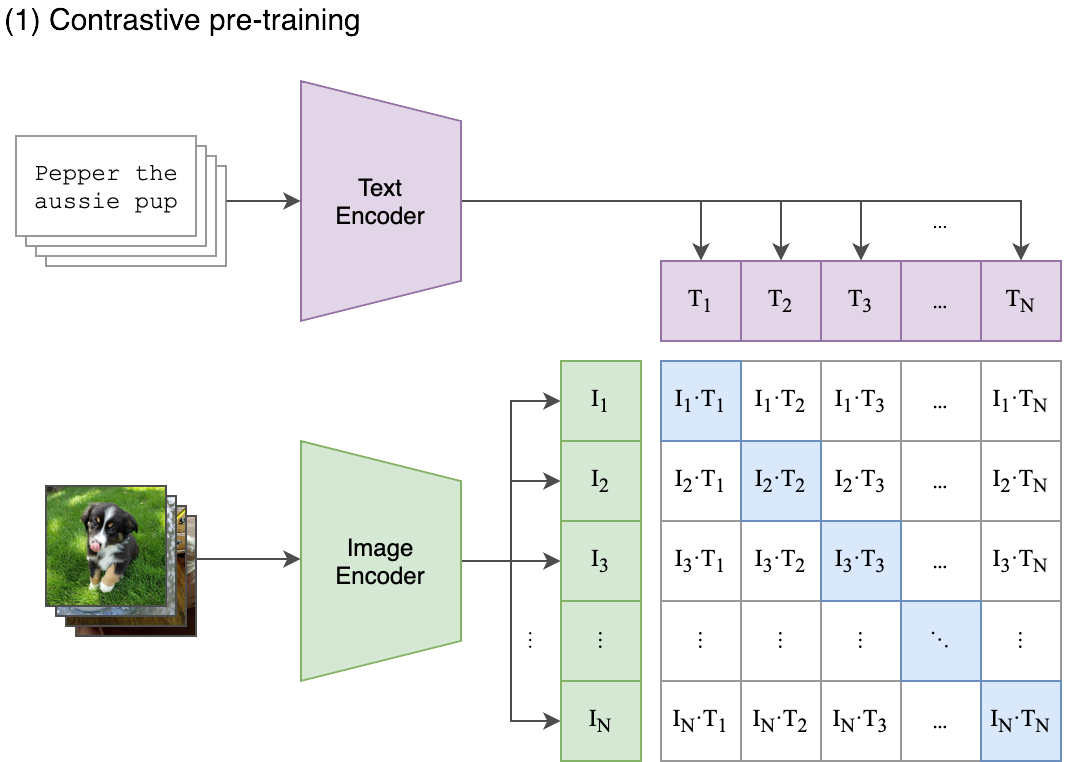
\includegraphics[scale=0.5]{./Slike/CLIP_arhitektura.png}
    \caption{Interakcija slikovnog i tekstualnog kodera CLIP-a. Preuzeto iz~\cite{radford2021learning}.}
    \label{fig:CLIP_architecture}
\end{figure}

\subsection{Okvir učenja}

Kada govorimo o CLIP-u kao okviru učenja, tada govorimo o okviru za multimodalno samonadzirano kontrastno učenje.\ Cilj učenja je naučiti i istovremeno uskladiti ugrađivanja dviju modalnosti.\ 
Kako bismo ovo postigli, prilikom učenja slikovnog i tekstualnog kodera želimo maksimizirati sličnost ugrađivanja slika i njihovih odgovarajućih opisa.\ Dodatno, želimo i minimizirati sličnost ugrađivanja krivo uparenih slika i opisa.\ 
CLIP za učenje ovog zadatka koristi infoNCE gubitak primijenjen dvosmjerno.\ CLIP gubitak možemo prikazati jednadžbom: 

\begin{equation}
    L_{CLIP} = - \frac{1}{2N} \sum_{j=1}^{N} \log{\frac{\exp(\langle \bm{z}_{j}^I, \bm{z}_{j}^T \rangle / \tau)}{\sum_{k=1}^{N}{\exp(\langle \bm{z}_{j}^I, \bm{z}_{k}^T \rangle / \tau)}}} - \frac{1}{2N} \sum_{k=1}^{N} \log{\frac{\exp(\langle \bm{z}_{k}^I, \bm{z}_{k}^T \rangle / \tau)}{\sum_{j=1}^{N}{\exp(\langle \bm{z}_{j}^I, \bm{z}_{k}^T \rangle / \tau)}}}
    \label{eq:CLIP_loss}
\end{equation}

Pritom $\bm{z}_{j}^I$ označava slikovno ugrađivanje slike primjera $\bm{x}_{j}^I$, $\bm{z}_{j}^T$ tekstualno ugrađivanje opisa primjera $\bm{x}_{j}^T$, a $\tau$ parametar temperature.\ 
Kao i prije, oznaka $\langle ... \rangle$ označava skalarni produkt elemenata unutar zagrada.\ 
CLIP gubitak sastoji se od dvije komponente jer želimo imati simetričnu usklađenost ugrađivanja slika i teksta u zajedničkom metričkom prostoru.\

\section{\textit{Zero-shot} klasifikacija}

\textit{Zero-shot} klasifikacija~\cite{xian2018zero} zadatak je dubokog učenja kod kojeg model na ulaz dobiva primjere iz neviđenih razreda te treba predvidjeti njihove oznake tj.\ razrede.\ 
Modeli učeni multimodalnim samonadziranim učenjem poput CLIP-a pogodni su za ovaj zadatak, no zahtijevaju dodatne informacije kako bi ga mogli obavljati.\

Na slici~\ref{fig:CLIP_zero_shot} možemo vidjeti kako se provodi \textit{zero-shot} klasifikacija kod CLIP-a.\ 
Kako bi CLIP mogao predvidjeti jedan od neviđenih razreda, na ulaz tekstualnog kodera dobiva opise u koje su ugrađena imena mogućih razreda.\ 
Za svaki od opisa izračuna se pripadno ugrađivanje te se ono usporedi s ugrađivanjem željene slike.\ Predviđeni razred je onaj za koji je sličnost pripadnog tekstualnog ugrađivanja sa slikovnim ugrađivanjem najveća.\

\begin{figure}[h]
    \centering
    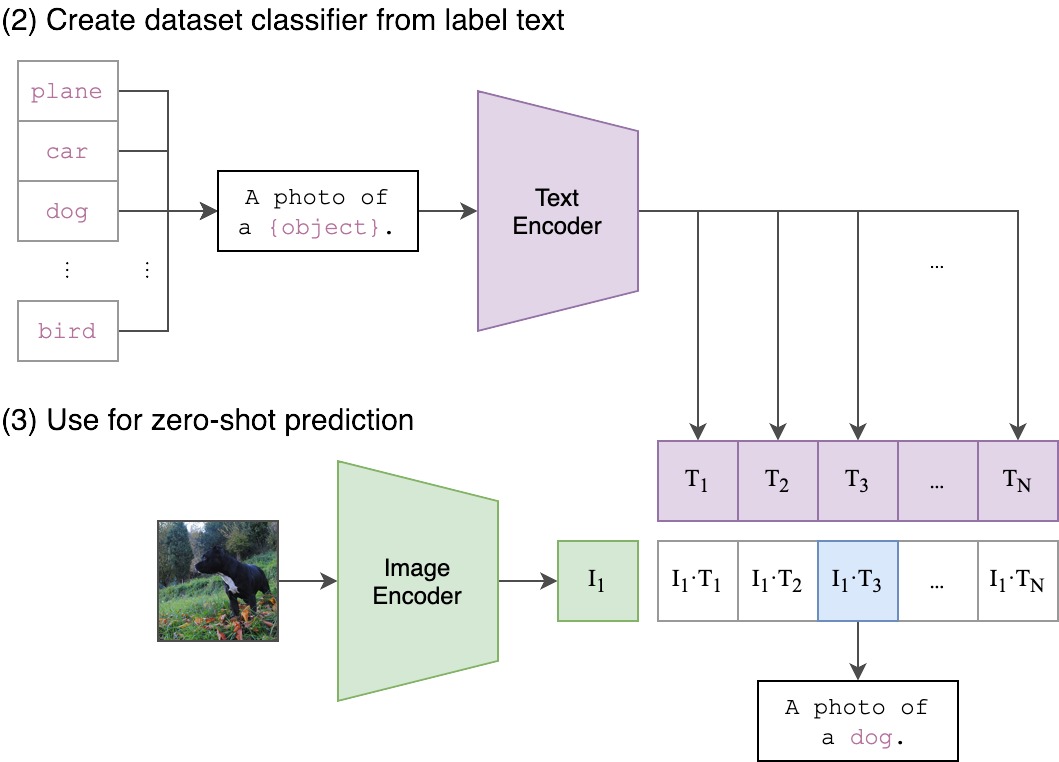
\includegraphics[scale=0.5]{./Slike/CLIP_zero_shot.png}
    \caption{\textit{Zero-shot} klasifikacija kod CLIP-a. Preuzeto iz~\cite{radford2021learning}.}
    \label{fig:CLIP_zero_shot}
\end{figure}

\chapter{Modeli mješavine}

\section{Općenito o modelima mješavine}

Modeli mješavine~\cite{lindsay1995mixture} vjerojatnosni su modeli koji modeliraju distribuciju ulaznih podataka.\ 
Glavna pretpostavka je da se distribucija podataka može modelirati kao linearna kombinacija niza jednostavnijih distribucija poput normalne ili Poissonove distribucije.\ 
Ove jednostavnije distribucije zovemo komponente modela mješavine.\ Uobičajeno sve komponente odgovaraju istoj vrsti parametrizirane distribucije.\ 
  
Osim ulaznih podataka $\bm{x}$, pretpostavljamo da postoji i diskretna latentna varijabla $z$.\ Realizacija latentne varijable $z$ određuje koja komponenta je generirala pripadni ulazni podatak.\ 
Distribuciju ulaznih podataka definiranu modelom mješavine možemo prikazati kao:

\begin{equation}
    p_{\bm{\theta}}(\bm{x}) = \sum_{k=1}^{K} p_{\bm{\theta}}(\bm{x}, z_k) = \sum_{k=1}^{K} p_{\bm{\theta}}(\bm{x}|z_k) \cdot p_{\bm{\theta}}(z_k)
    \label{eq:mixture_model}
\end{equation}

Pritom $p_{\bm{\theta}}(\bm{x})$ označava distribuciju ulaznih podataka, $p_{\bm{\theta}}(\bm{x}, z_k)$ zajedničku distribuciju ulaznih podataka i latentne varijable, $p_{\bm{\theta}}(\bm{x}|z_k)$ \textit{k}-tu komponentu mješavine tj.\ uvjetnu distribuciju ulaznih podataka uz realizaciju latentne varijable, a $p_{\bm{\theta}}(z_k)$ težinu \textit{k}-te komponente tj.\ distribuciju latentne varijable.\
  
Parametri modela mješavine uobičajeno se uče algoritmom maksimizacije očekivanja (engl.\ expectation-maximization algorithm)~\cite{moon1996expectation}.\ 
Algoritam maksimizacije očekivanja iterativan je algoritam koji se često koristi za učenje parametara modela s latentnim varijablama.\ 
U svakoj iteraciji, algoritam alternira između koraka procjene očekivanja log-izglednosti uz fiksirane parametre i koraka ažuriranja parametara tako da isti maksimiziraju izračunato očekivanje.\ 

\section{Model Gaussove mješavine}

Model Gaussove mješavine~\cite{reynolds2009gaussian} vrsta je modela mješavine kod koje komponente modeliramo normalnom distribucijom.\
Drugim riječima, pretpostavka je da su ulazni podatci generirani iz normalne distribucije s parametrima $\bm{\mu}_k$ i $\bm{\Sigma}_k$.\ 
Pritom, $\bm{\mu}_k$ te $\bm{\Sigma}_k$ označavaju vektor srednjih vrijednosti i kovarijacijsku matricu \textit{k}-te komponente.\
Distribuciju ulaznih podataka tada možemo prikazati jednadžbom:

\begin{equation}
    p_{\bm{\theta}}(\bm{x}) = \sum_{k=1}^{K} p_{\bm{\theta}}(z_k) \cdot \mathcal{N}(\bm{x}|\bm{\mu}_k, \bm{\Sigma}_k)
    \label{eq:gaussian_mixture_model}
\end{equation}

Kao i prije, $p_{\bm{\theta}}(\bm{x})$ označava distribuciju ulaznih podataka, $p_{\bm{\theta}}(z_k)$ distribuciju latentne varijable, a $\mathcal{N}(\bm{x}|\bm{\mu}_k, \bm{\Sigma}_k)$ \textit{k}-tu komponentu mješavine.\ 
  
Na slici~\ref{fig:GMM} možemo vidjeti primjer modela Gaussove mješavine s tri komponente.\ Plavom, zelenom i narančastom bojom označene su pojedine komponente skalirane pripadnim težinama, dok je crtkanom linijom označen konačni model distribucije ulaznih podataka.\

\begin{figure}[h]
    \centering
    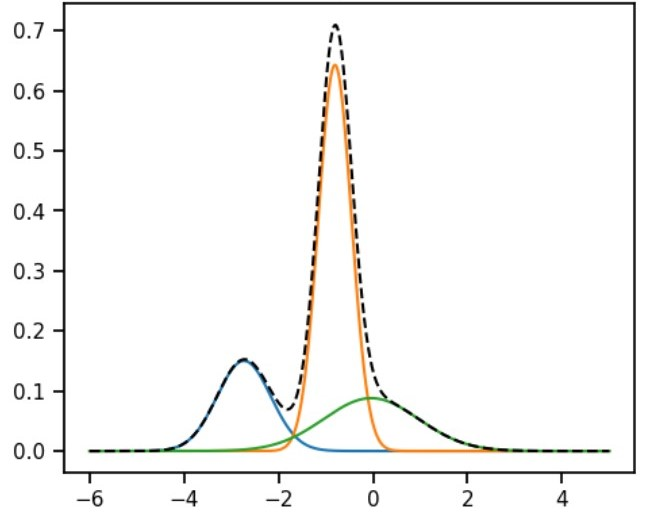
\includegraphics[scale=1]{./Slike/GMM.jpg}
    \caption{Primjer modela Gaussove mješavine.}
    \label{fig:GMM}
\end{figure}

\chapter{Napadi na modele strojnog učenja}

\section{Trovanje podataka}

Trovanje podataka vrsta je napada kod kojeg napadač ima pristup skupu za učenje i u njega ubacuje zatrovane podatke.\
Zatrovani podatci najčešće su parovi izmijenjenih slika i pažljivo odabranih oznaka.\ 
Izvorne slike za učenje mijenjaju se tako da im se doda okidač~\cite{chen2017targeted}.\ 
Okidač može biti ograničen na mali dio slike, ali i protezati se preko cijele slike.\
  
Najjednostavniji cilj trovanja podataka je pogoršanje dobrote naučenih modela.\ Ipak, napadač od takvog trovanja nema puno koristi.\
Puno opasniji cilj je ugrađivanje stražnjih vrata u model.\ Ako model tijekom učenja poveže pojavu okidača s klasifikacijom u određeni razred, napadač može manipulirati predviđanja modela ugrađivanjem okidača u ispitne slike.\
Ovakvu vrstu napada zvat ćemo trojanski napad.\

\section{Trojanski napad na multimodalne modele}

Trojanski napad na multimodalne modele koji uče na parovima slika i njihovih opisa djelomično se razlikuje od "klasičnog" trojanskog napada.\ 
Izvorne slike za učenje i dalje se mijenjaju dodavanjem okidača.\ Na slici~\ref{fig:image_poisoning} možemo vidjeti primjer izmjene slike iz skupa ImageNet1K.\ 
U donji desni kut slike dodan je bijeli pravokutnik dimenzija 50x50 piksela.\ Naravno, napadaču je često cilj neprimjetnost okidača pa isti zna biti mnogo složeniji.\

\pagebreak

\begin{figure}[h]
    \centering
    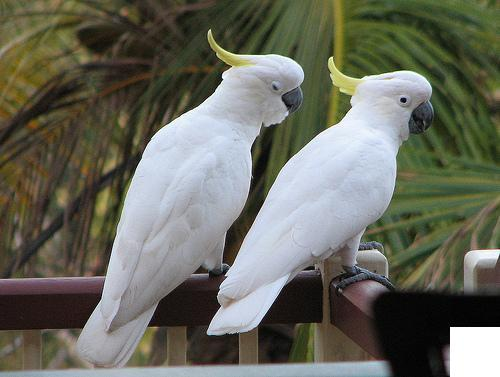
\includegraphics[scale=0.6]{./Slike/image_poisoning.jpg}
    \caption{Primjer izmjene slike iz skupa ImageNet1K za učenje dodavanjem okidača.}
    \label{fig:image_poisoning}
\end{figure}

Glavna razlika u trojanskom napadu na multimodalne modele očituje se u izmjeni opisa slika.\ 
Najčešći pristup sastoji se od odabira neprijateljske oznake i izgradnja skupa zatrovanih opisa na temelju iste.\ 
  
U prvom koraku izmjene opisa, napadač bira neprijateljsku oznaku.\ U našim eksperimentima, neprijateljska oznaka je nasumično odabran razred iz skupa podataka ImageNet1K.\ 
Sljedeći korak je izgradnja skupa zatrovanih opisa.\ Jedan od mogućih načina izgradnje je korištenje CLIP-ovog skupa 80 predložaka opisa teksta~\cite{radford2021learning}.\ 
Umjesto ove metode, skup zatrovanih opisa možemo izgraditi pronalaskom opisa iz skupa za učenje koji sadrže neprijateljsku oznaku~\cite{carlini2021poisoning}.\
  
Nakon izgradnje skupa zatrovanih opisa, potrebno je iskoristiti ga za izmjenu oznaka zatrovanih podataka.\ 
Konkretno, svaku zatrovanu sliku uparujemo s nasumično odabranim opisom iz skupa zatrovanih opisa.\ 
Na kraju ovoga postupka imamo skup parova zatrovanih slika i zatrovanih opisa koje ubacujemo u prirodni skup za učenje.\

\chapter{Obrana od napada}

\section{Općenito o obranama od napada}

Ako znamo koji su podatci zatrovani, uspješnost napada možemo mjeriti stopom uspješnosti napada (engl. \textit{attack success rate - ASR}).\ 
Glavni cilj algoritama za obranu od napada je otklanjanje ranjivosti modela bez narušavanja performansi na prirodnim podatcima.\ 
Otklanjanje nesigurnosti modela možemo poistovjetiti sa smanjivanjem stope uspješnosti napada.\ Drugim riječima, cilj obrane je smanjiti iznos ASR-a, ali i istovremeno zadržati otprilike jednak iznos standardnih mjera dobrote.\ 
  
Iako se pokazuje da je CLIP veoma ranjiv na napade~\cite{carlini2021poisoning}, ne postoji velik broj obrana za multimodalne modele.\ 
Općenito govoreći, algoritmi obrane mogu se kategorizirati u dvije skupine.\ 
Prva skupina algoritama bavi se čišćenjem već zatrovanog modela, dok se druga skupina bavi aktivnom obranom modela tijekom učenja.\ 
Primjeri aktivne obrane modela su RoCLIP~\cite{yang2023robust} i SafeCLIP~\cite{yang2023better}.\

\section{SafeCLIP}

Algoritam obrane SafeCLIP nastoji otkloniti ranjivost modela razdvajanjem skupa za učenje u sigurni i nesigurni skup.\ 
Učenje na sigurnom skupu provodi se koristeći CLIP gubitak, dok se učenje na nesigurnom skupu provodi primjenom unimodalnog tj.\ infoNCE gubitka zasebno na slike odnosno opise slika.\ 
SafeCLIP se sastoji od tri glavne faze učenja: 

1.\ unimodalno kontrastno zagrijavanje
  
2.\ primjena CLIP gubitka uz smanjenu stopu učenja   
  
3.\ učenje s CLIP gubitkom i unimodalnim gubitkom  

\pagebreak

\subsection{Unimodalno kontrastno zagrijavanje}

U prvoj fazi učenja, glavni cilj je postići grupiranje ugrađivanja sličnih slika, kao i sličnih opisa, u zajedničkom metričkom prostoru.\ 
Tijekom svake epohe ove faze, model zasebno uči na skupu svih slika, kao i na skupu svih opisa.\ 
Učenje se provodi koristeći infoNCE gubitak uz korištenje standardnih perturbacija slika te tekstualnih opisa.\  
  
Pošto se učenje provodi odvojeno na slikama odnosno na opisima, tijekom ove faze nije moguće zatrovati model.\ 
Na kraju faze, slične slike, kao i slični opisi, nalazit će se relativno blizu u metričkom prostoru.\ Istovremeno, zbog zasebnog učenja svakog modaliteta, ugrađivanja slika i njihovih pripadnih opisa neće nužno biti bliska.\ 
  
Kako bi se dodatno poboljšala kvaliteta ugrađivanja, kao i smanjila vjerojatnost bliskog grupiranja slika i njihovih zatrovanih verzija, infoNCE gubitak može se izmijeniti.\ 
Konkretno, umjesto uparivanja ugrađivanja sidra s ugrađivanjem pozitiva odnosno negativima, uparujemo najbližeg susjeda ugrađivanja sidra.\ 
Drugim riječima, u jednadžbi infoNCE gubitka ugrađivanje sidra zamijenjeno je s najbližim ugrađivanjem iz ograničenog skupa tj. bazena ugrađivanja.\ 
Izmijenjeni gubitak zvat ćemo unimodalni gubitak, a možemo ga prikazati jednadžbom:

\begin{equation}
    L_{unimodal} = - \log{\frac{\exp(\langle NN(\bm{z}_{a}, \mathcal{P}), \bm{z}_{p} \rangle / \tau)}{\sum_{i=1}^{N}{\exp(\langle NN(\bm{z}_{a}, \mathcal{P}), \bm{z}_{ni} \rangle / \tau)}}}
    \label{eq:unimodal_loss}
\end{equation}

Pritom $\bm{z}_{a}$ označava ugrađivanje sidra $\bm{x}_{a}$, $\bm{z}_{p}$ ugrađivanje pozitivnog primjera $\bm{x}_{p}$, $\bm{z}_{ni}$ ugrađivanje i-tog negativnog primjera iz minigrupe $\bm{x}_{ni}$, a $\tau$ parametar temperature.\ 
$NN(\bm{z}_{a}, \mathcal{P})$ označava najbližeg susjeda tj.\ najbliže ugrađivanje iz trenutnog bazena ugrađivanja, a oznaka $\langle ... \rangle$ označava skalarni produkt elemenata unutar zagrada.\

\subsection{Primjena CLIP gubitka uz smanjenu stopu učenja}

Na kraju prethodne faze, ugrađivanja slika i pripadnih opisa neće nužno biti bliska u metričkom prostoru.\ 
Kako bismo mogli prepoznati potencijalno zatrovane parove i razdvojiti skup za učenje u sigurni odnosno nesigurni skup, potrebno je malo približiti ugrađivanja slika i opisa.\
  
Provođenjem učenja koristeći CLIP gubitak približit će se ugrađivanja slika i opisa.\ 
U ovom koraku veoma je važan odabir prikladne stope učenja.\ Odabirom prevelike stope učenja dolazi do opasnosti trovanja modela, dok odabir premale stope učenja neće dovoljno približiti ugrađivanja.\ 
Pokazuje se da učenje s uobičajenom stopom učenja skaliranom faktorom iznosa $0.01$ dovoljno približava ugrađivanja bez trovanja modela.\
  
Nakon učenja koristeći CLIP gubitak uz smanjenu stopu učenja, moguće je podijeliti skup za učenje u sigurni odnosno nesigurni skup.\ 
Prvi korak je izračun kosinusne sličnosti slika i pripadnih opisa.\ Pritom očekujemo da će zatrovani parovi imati veoma nisku sličnost, dok će ispravni parovi imati višu sličnost.\ 
Sljedeći korak je učenje modela Gaussove mješavine s dvije komponente koristeći kosinusne sličnosti kao ulazne podatke.\ Za svaki par slika i njihovih opisa izračuna se vjerojatnost pripadnosti komponenti Gaussove mješavine s većom srednjom vrijednosti.\ 
Svi parovi za koje je vjerojatnost pripadnosti iznad određenog praga, npr. $t = 0.9$, proglašavaju se sigurnima, dok se preostali parovi smatraju nesigurnima.\ 
Ovakvim postupkom osiguravamo da se većina zatrovanih primjera nalazi u nesigurnom skupu.\ 

\subsection{Učenje s CLIP gubitkom i unimodalnim gubitkom}

Posljednja faza SafeCLIP algoritma je učenje modela s CLIP gubitkom i unimodalnim gubitkom.\ 
Parovi iz sigurnog skupa koriste se za učenje s CLIP gubitkom, dok se parovi iz nesigurnog skupa koriste za učenje s unimodalnim gubitkom.\ 
Drugim riječima, ako par pripada sigurnom skupu, želimo naučiti ugrađivanje koje će približiti sliku i pripadni opis.\ 
Ako par pripada nesigurnom skupu, želimo naučiti zasebno slikovno odnosno tekstualno ugrađivanje.\ Ovim načinom tijekom učenja koristimo cijeli skup, time smanjujući rizik od lošijih performansi na prirodnim podatcima.\ 
  
Nakon svake epohe ove faze, ponovno se provede postupak izračuna sličnosti parova, kao i podjele u sigurni odnosno nesigurni skup.\ 
Pritom je važno istaknuti da se svaku epohu povećava dopušten broj parova u sigurnom skupu za $1\%$.\
Posljedično, u zadnjim epohama učenja će sigurni skup sadržavati gotovo sve parove, dok će nesigurni skup biti veoma malen.\ 
Ukupni gubitak učenja s CLIP gubitkom i unimodalnim gubitkom možemo prikazati jednadžbom:

\begin{equation}
    \mathcal{L}_{SafeCLIP}(\mathcal{D}) = \mathcal{L}_{CLIP}(\mathcal{D}_{safe}) + \mathcal{L}_{unimodal}(\mathcal{D}_{unsafe})
    \label{eq:total_loss}
\end{equation}

Pritom $\mathcal{D}$ označava cijeli skup podataka, $\mathcal{D}_{safe}$ sigurni skup, a $\mathcal{D}_{unsafe}$ nesigurni skup.\

\chapter{Skupovi podataka}

\section{CC3M}

Skup CC3M (engl.\ \textit{Conceptual Captions 3 Million})~\cite{sharma2018conceptual} sastoji se od otprilike 3.3 milijuna slika i pripadnih opisa.\ 
Slike i njihovi opisi prikupljeni su s Interneta, a prikazuju razne scene i objekte iz svakodnevnice.\ Za prikupljanje opisa korišten je \textit{Alt-text} HTML atribut asociran sa slikama na Internetu.\ 
Parovi slika i opisa dodatno su filtrirani i transformirani kako bi se postigla uravnoteženost čistoće, jasnoće i informativnosti opisa.\ Postupak filtriranja i transformiranja u potpunosti je automatiziran.\ 

Na slici~\ref{fig:CC3M} možemo vidjeti dva primjera slika i opisa iz skupa CC3M.\ Dodatno, na slici možemo vidjeti i originalne \textit{Alt-text} HTML atribute na temelju kojih su nastali pripadni opisi.\
Konačni opisi puno sažetije opisuju pripadnu sliku u usporedbi s \textit{Alt-text} HTML atributima.\

\begin{figure}[h]
    \centering
    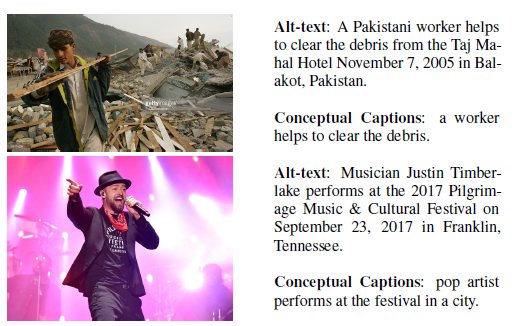
\includegraphics[scale=0.7]{./Slike/CC3M.png}
    \caption{Primjer slika i opisa iz skupa CC3M. Preuzeto iz~\cite{sharma2018conceptual}.}
    \label{fig:CC3M}
\end{figure}

\section{ImageNet1K}

Skup ImageNet1K najčešće je korišteni podskup skupa ImageNet~\cite{deng2009imagenet}.\ 
Podijeljen je na 1 281 167 slika u skupu za učenje, 50 000 slika u skupu za validaciju i 100 000 slika u skupu za ispitivanje.\ 
Svaka od slika može pripadati jednom od ukupno 1000 razreda.\ Pojedini razredi predstavljaju različite koncepte, od životinja pa sve do različitih vrsta igračaka.\ 
Podskup ImageNet1K godinama se koristio za evaluaciju algoritama za klasifikaciju i detekciju objekata u sklopu natjecanja ILSVRC (engl.\ \textit{mageNet Large Scale Visual Recognition Challenge}).\
  
Slika~\ref{fig:imagenet} prikazuje nekoliko slika i razreda iz skupa ImageNet.\ Skup podataka strukturiran je hijerarhijski.\ Slike iz razreda \texttt{husky} također pripadaju i u razrede \texttt{dog} te \texttt{mammal}.\

\begin{figure}[h]
    \centering
    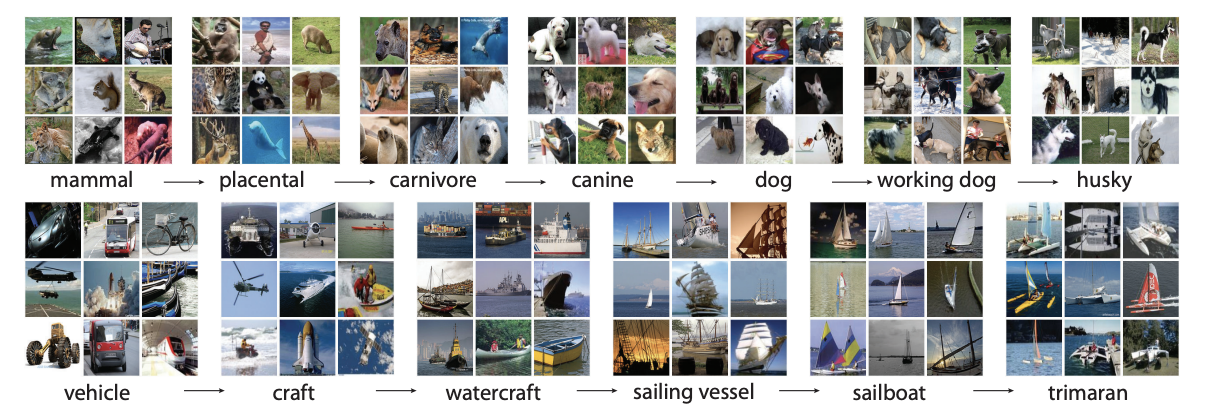
\includegraphics[scale=0.33]{./Slike/imagenet.png}
    \caption{Primjer slika i razreda iz skupa ImageNet. Preuzeto iz~\cite{deng2009imagenet}.}
    \label{fig:imagenet}
\end{figure}

\chapter{Eksperimenti}

Eksperimenti.

\chapter{Zaključak}

Zaključak.

\bibliography{literatura}
\bibliographystyle{fer}

\chapter{Sažetak}
Sažetak.

\end{document}
